\chapter{Conclusions} \label{chap:conclusions}

In conclusion, this report establishes a solid foundation for implementing and proposing concrete improvements to \ac{GRL} techniques and efficiently solve the problem of \ac{DED} in graph-based environments. \par
We concluded in the literature review, that \ac{GRL} is already a promising solution for \ac{DED}, yielding better performance than other approaches. In general, \acp{GNN} are an ubiquitous method, throughout the gathered literature, for extracting efficient environment topological representations. The identified limitations of existent implementations lie on their lack of: (1) scalability to larger environments, resulting in a significant decrease in computation performance; (2) a seamless integration between \ac{GNN} and \ac{DRL} algorithms and (3) adaptability to real-time topology changes. \par
Moreover, we aim to study how to tackle these limitations by implementing different \ac{GRL} approaches for solving the \ac{DED} problem and conducting a comparative study between the different techniques. The implementations will be compromised of various combinations of \acp{GNN}, for efficiently extracting the relevant environment features, and \ac{DRL} algorithms for mapping the extracted representations into optimal action sequences. Case studies will be carried out within different size modified IEEE bus systems for testing the various models and confront their results. Lastly, the models will be analysed considering their training efficiency, computational performance, dispatch efficiency, scalability to large scenarios and adaptability to topological changes. Based on the conclusions drawn from the comparative study, we will propose a \ac{GRL} that implements concrete enhancements.

\section{Expected Contributions}

In this section, we list the expected contributions derived from this work on a Scientific, Technological and Application levels:
\begin{description}
	\item[Scientific] A systematic and comparative study of different GRL approaches. This fills the research gap for systematic studies comparing different proposed techniques. Furthermore, this work will bring a clearer insight regarding the best practices on implementing \ac{GRL} models
	\item[Technological] A model resulting from this study with concrete improvements over the current GRL techniques proposed so far and tackling their limitations. Beyond this, 
	\item[Application] An efficient solution for the DED problem with GRL algorithms, compromising significant contribution to the research on \ac{DED} systems on complex scenarios
\end{description}

\section{SWOT Anaysis}

\begin{figure}[H]
	\centering
	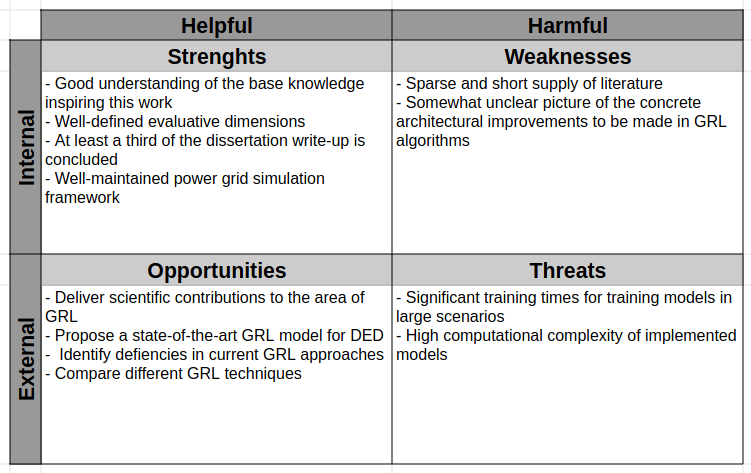
\includegraphics[width=0.90\linewidth]{./figures/swot.png}
	\caption{SWOT Analysis}
	\label{fig:swot}
\end{figure}

\section{SMART Analysis}

Lastly, we formulated this disseration's objectives considering the criteria imposed by SMART goals. Recapitulating from chapter \ref{chap:intro}:
\begin{enumerate}
	\item Perform a review of literature regarding \ac{GRL} approaches and \ac{DED} systems
	\item Conduct a comparative and systematic empirical study of different \ac{GRL} solutions of the \ac{DED} problem
	\item Propose a \ac{GRL} model and concrete improvements facing the literature proposed models
\end{enumerate}

In this manner, we analyse these goals from the SMART perspective to ensure that they represent a clear road map for conducting this study. Considering each dimension of the SMART criteria, we conclude that the defined objectives are:

\begin{description}
	\item[Specific] All of the goals refer to a concrete objective of this work and are further specified in the proposed work plan (figure \ref{fig:gantt-chart})
	\item[Measurable] The progress towards each objective is measurable
	\item[Achievable] The objectives are realistic and attainable, considering the already existent research
	\item[Relevant] Objectives 1 and 2 enable a better foundation for accomplishing the third objective, which compromises the main goal of this dissertation
	\item[Time-bound] All of the objectives are time-bound by the proposed work plan in figure \ref{fig:gantt-chart}, divided into more specific tasks.
\end{description}

